\chapter{Literature Review}
\label{chapter:literatureReview}

Before we begin the actual development of our anomaly detection tool, we first needed to establish some core concepts and review the good work that has already been done in this area.

Therefore, in the following sections, we will introduce the notion of anomaly detection. We will present ideas that the reader should be familiar with in order to fully understand anomaly detection techniques and, by extension, our work.

We then explain the three main categories of machine learning - supervised, semi-supervised and unsupervised. We discuss what their distinctive features are when applied in the anomaly detection domain. 
We then go into detail about four different machine learning algorithms and argue why they are the most suitable candidates for our task.

We also explain what we understand by a log, log template, and discuss the most common techniques for log parsing and log-template mining.

We conclude the chapter with an analysis of various log parsing tools. The overview allows us to argue which log parser would be best suited for our application.

\section{Anomaly Detection}
\label{section:anomalyDetectionLiteratureReview}

% The definition of anomaly detection
\textit{Anomaly detection} is a problem of finding patterns in data that do not follow the expected normal behaviour represented by the majority of data points. It follows that defining the normal behaviour is one of the crucial challenges of anomaly detection. 
The unusual patterns are also called \textit{outliers} or \textit{anomalies} and anomaly detection is often called \textit{outlier detection}. 
Outlier was defined by Ord \cite{ORD1996175} as an outlying observation that appears to be significantly different from other members of the sample in which it occurs. 
In other words, the statistical properties of the anomalous data points are not in alignment with the rest of the data. 
Outliers vary by domain and can occur for a variety of reasons, such as fraudulent behaviour in credit card fraud, computer network intrusions, system failures, mechanical failures in industrial applications, deviations due to natural behaviour, or human error. 

Anomaly detection is also related to the term \textit{noise}. Noise is defined as an undesirable phenomenon in data that is not of interest to the analyst but hinders data analysis \cite{cvbakv2009}. Noise is caused by an external factor unrelated to the distribution that generates the data \cite{ggh2017} and leads to excessively complex models with degraded performance \cite{wu2007}. 

In our thesis, we focus on anomaly detection in \textit{time series} data. Time series outlier analysis examines anomalies in the behaviour of data over time \cite{gupta2014}. An outlier in time series data is a data point that does not follow a common behaviour, either a general long-term trend or a tendency of the data to increase or decrease in seasonal patterns.

Originally, outliers were detected manually by the hand of a domain expert. 
Nowadays, the focus of anomaly detection is on automatic detection of anomalous behaviour. 
It has been proven on many occasions that the problem of automatic anomaly detection can be successfully tackled by learning from data \cite{he2016} \cite{wang2017timeseriesanomaly}.
\\
We can divide anomaly detection methods into three broad categories: \textit{supervised}, \textit{semi-supervised} and \textit{unsupervised} anomaly detection. Supervised learning algorithms are trained by examples and require a dataset that is already labeled. Unsupervised methods, on the other hand, do not require any labeled data at all. Semi-supervised methods combine both approaches; in addition, some semi-supervised approaches assume that normal class instances are labeled.

% describe the advantages of unsupervised methods over supervised ones https://reader.elsevier.com/reader/sd/pii/S0167404818306333?token=9C7DC222C83AC3AD33CBF921C2E23508BEA68B59C5336EC0200EF02A1F60DAB2916EEE9D83663EE9029AB30B9C1CC538

\subsection{Supervised Anomaly Detection}
Supervised methods require previously labeled data, where the labels describe whether the behaviour in each data instance is normal or abnormal (anomalous). The main focus of supervised learning methods is then to derive a model from the labeled data that maximizes the discrimination between the classes (normal and anomalous). A drawback of the supervised method is that it can only be trained on the types of anomalies introduced in the training examples. It cannot handle previously unseen anomalies. 

\subsection{Semi-supervised Anomaly Detection} %https://www-users.cs.york.ac.uk/vicky/myPapers/Hodge+Austin_OutlierDetection_AIRE381.pdf.
%https://researchbank.swinburne.edu.au/file/cee84793-6f09-49ce-a099-41451c803b81/1/mostafa_farshchi_thesis.pdf
Semi-supervised learning is defined as a machine learning paradigm that studies how computers, or even natural systems like humans, learn in the presence of both labeled and unlabeled data \cite{zhu2009introduction}.

 
\subsection{Unsupervised Anomaly Detection}
Unsupervised learning, unlike supervised learning, does not require any prior knowledge about the data. One of the main difficulties faced by anomaly detection is unlabeled data. In most cases, logs with labeled anomalies are not available. The process of log annotation would have to be done manually by the experts - developers who are familiar with the system. Along with the growth of data volume, labeling becoms very time consuming. For this reason, in practice, anomaly detection mostly relies on unsupervised learning to deal with unlabeled data. Unsupervised anomaly detection algorithms learn what normal behaviour looks like. Based on these observations, systems based on unsupervised methods detect anomalies as outliers that are significantly different from other examples. Moreover, any type of anomaly can be detected by these systems. Thus, the main difference between supervised and unsupervised learning techniques is that the former focuses on discriminating concept classes, while the latter rather focuses on data characterization \cite{Goernitz_2013}. % They work on the basis of the observation that an abnormal instance usually manifests as an outlier point that is distant from other instances. As such, unsupervised learning techniques, such as clustering, can be applied.
 
\subsubsection*{One-Class Classification}
When it comes to anomaly detection, it is common to use a special method called One-Class Classification (or One-Class Learning) formulated by Tax \cite{tax2002occ}. 
 
In OCC, labels are only provided for instances of the normal class, while labels are not required for classes describing anomalies. In fact, it is discouraged that they occur in the training dataset. There should be so few instances of outliers that they do not form a statistically representative sample of the negative concept \cite{khan_madden_2014}.
 
Thus, in a semi-supervised mode, the model that captures normal behaviour is created and used to identify anomalous behaviour. A class describing normal data is used primarily because it is more readily available, while a labeled dataset that would cover all anomalies is difficult to obtain \cite{cvbakv2009}.
 
Due to the nature of our data, we used unsupervised anomaly detection methods for this study.

\subsubsection{Isolation Forest}
\label{section:lrIsolationForest}
Isolation Forest or iForest \cite{liu2012isolation} is an ensemble approach for anomaly detection. Majority of existing model-based methods attempt to model normal behaviour, and then a deviation from the normal region that does not fit the model well is considered an anomaly \cite{introToDataMining2005}. Isolation Forest approach, on the other hand, isolates anomalies directly without using the distance from the previously defined normal region. It exploits two properties that can be observed in anomalies. Anomalous instances are the minority of data points and their attribute-values are very different from normal instances. Due to these properties, anomalies are susceptible to a concept called \textit{isolation}, which is the main idea behind Isolation Forests. Liu et al. \cite{liu2012isolation} defined isolation in their research paper as "separation of an instance from the rest of the instances".

Isolation Forest starts by selecting a random attribute and then creates a random partition between the maximum and minimum values of that attribute. This process is applied recursively until all samples are isolated, which can be represented by a binary tree structure (Isolation Tree of iTree). Then, the number of partitions performed to isolate a point is equal to the length of the traversal path from the root node to a terminating node. The iForest is built by adding a given number of iTrees obtained by randomly generated partitions, and their averaged traversal path lengths are then used as a measure of anomaly score. It is easy to see that the isolation of anomaly instances happens closer to the root of the tree, hence the path lengths are also shorter.

Since the anomaly score is the average path length of iTree, which corresponds to an unsuccessful search in the binary search tree, the equation for the anomaly score is derived from the analysis of the binary search tree. Let $n$ be the number of instances in a dataset $X$. The anomaly score $s$ of an instance $x \in X$ is defined as:
 
 \begin{gather}
     s(x, n) = 2^{- \dfrac{E(h(x))}{c(n)}},
 \end{gather}
 
 where $h(x)$ a length of a traversed path from the root node to a terminating node $x$, $E(h(x))$ is the average of $h(x)$ in all isolation trees and $c(n)$ is a normalization factor defined as: 
 
 \[
 c(n) = 
  \begin{dcases}
     c(n) = 2H(n - 1) - (2(n - 1) / n), & \text{if} n > 2\\
     1, & \text{if} n = 2\\
     0, & \text{otherwise}
 \end{dcases} 
 \]
 
where $H(i)$ is the harmonic number estimated by $ln(i) + 0.5772156649$. \\

The Isolation Forest algorithm operates in linear time complexity and is particularly suitable for large and high dimensional datasets due to its low memory requirements. It is proven to be an accurate and effective anomaly detector.

\subsubsection*{Anomaly Detection Forest}
Recently, a variant of the Isolation Forest algorithm has been studied for the specific use case of Anomaly Detection - Anomaly Detection Forest \cite{adForest}. It is also commonly referred to as One-Class Isolation Forest. 
It falls under the category of One-Class Classification algorithms.

Sternby et al. claim that the algorithm outperforms the state-of-the-art algorithms Isolation Forest and One-Class Random Forest for the task of anomaly detection in the one-class learning setting. They argue that IF has an intrinsic bias towards labeling similar unusual normal instances as anomalies \cite{adForest}.

They try to improve that by introducing two new concepts \cite{adForest}:
\begin{itemize}
    \item \textit{Anomaly leaves} with the aim of catching anomalies with feature values that are not contained
            in the range of the subsample of tree training observations.
    \item \textit{Isolation level}, which is a lower size bound on the training samples in a node during training, and determines when anomaly leaves should be created rather than further subdividing the training samples.
\end{itemize}

Although the results seem promising, we decided not to proceed with this algorithm because the reference implementation is proprietary.
Our goal is to optimize the original IF algorithm so that it performs reasonably well when learning from normal data only.
 
\subsubsection{PCA}
\label{section:lrPCA}
%https://www.usenix.org/legacy/event/sysml08/tech/full_papers/xu/xu.pdf
One problem with high dimensional data is that it is often noisy and even redundant. In such a case, dimensionality reduction is a useful tool to address this problem. Principal Component Analysis (PCA) is one of the most commonly used dimension reduction methods. The reduction is done by projecting the data onto a lower dimensional subspace that captures the "essence" of the data \cite{murphy2013machine}. The similarities and differences in the data become visible in the new coordinate system. 

PCA uses projection methods on a given set of input data points with many input features. Once a PCA model is obtained, a distance from test log entries (either positive or negative) to normal space can be calculated to detect anomalies. Correlations in the original feature space are searched for and the combination of variables that maximizes variance is found to preserve all information with minimal redundancy. A new, more representative and compact feature space is generated. This feature space with lower dimensions is called the \textit{principal components}. The features in the principal components are uncorrelated and ordered by the proportion of the data variance that each feature captures.\\

To put it formally, let's say we have an $m$-dimensional vector $\mathbf{Y} \in \mathbb{R^n}$ with $n$ standardized input features in the original data. The PCA model decomposes $\mathbf{Y}$ into two parts \cite{pca1997}:

\begin{gather}
 \mathbf{Y} = \mathbf{\hat{Y}} + \mathbf{\widetilde{Y}}
\end{gather}

Where $\mathbf{\hat{Y}}$ represents the modeled part of the projection - the selected principal components. $\mathbf{\widetilde{Y}}$ represents the residual part of the projection. The modeled part is obtained by projecting the original data $\mathbf{{Y}}$. The projection is shown in the equation \ref{formula:projection}, where $\mathbf{P} \in \mathbb{R}^{n \times k}$ is the PCA loading matrix, $k$ is the number of principal components, and the matrix $\mathbf{C = \mathbf{PP}^T}$ is a projection matrix. 
Thus, $\mathbf{C}$ is a matrix for a projection of the original data onto a model space, so called normal space $S_d$ with $n$ dimensions.

\begin{gather}
     \mathbf{\hat{Y}} = \mathbf{P}\mathbf{P}^T\mathbf{Y} = \mathbf{CY}
    \label{formula:projection}
\end{gather}

The remaining $(n - k)$ dimensions form the residual subspace, also called the anomaly space $S_a$. $\mathbf{\widetilde{Y}}$ corresponds to the projection of $\mathbf{Y}$ onto the residual subspace $S_a$. The equation \ref{formula:residualProjection} shows how the $\mathbf{\widetilde{Y}}$ can be mathematically computed.  

\begin{gather}
     \mathbf{\widetilde{Y}} = (\mathbf{I - C})\mathbf{Y} = \mathbf{\widetilde{C}Y}
    \label{formula:residualProjection}
\end{gather}
 
% How is it applied in anomaly detection.
When PCA is applied to an anomaly detection task, for each new input its projection is computed. An anomaly can be detected with a large change in variable correlation if normal behaviour is not preserved. If this is the case, the projection on the residual subspace $S_a$ is increased. As a side effect, unusual values of the magnitude of $\mathbf{\widetilde{Y}}$ can be observed. In other words, an anomalous vector is farther away from the normal space $S_d$.\\

The squared prediction error (SPE) in the equation \ref{formula:predictionError} is a useful evaluation metric to measure the distance from $S_d$.
 
 \begin{gather}
     SPE = \parallel \mathbf{\widetilde{Y}} \parallel^2  = \parallel \mathbf{\widetilde{C}Y} \parallel^2
    \label{formula:predictionError}
\end{gather}

SPE is used as an anomaly score: The higher the prediction error, the more anomalous the data instance. A process block is considered an anomaly if:

\begin{gather}
     SPE \leq \delta^2
\end{gather}

where $\delta^2$ is a threshold for the error. A standard implementation of the threshold  $\delta^2$ in anomaly detection is based on the \textit{Q-statistics} proposed by Jackson \cite{pcaJackson1979}. According to this, an anomaly is flagged if the following holds:

\begin{gather}
    SPE = \parallel \mathbf{\widetilde{Y}} \parallel^2 > Q_{\alpha} 
\end{gather}
 
where $Q_{\alpha}$ denotes a Q-value statistics providing a $(1 - \alpha)$ confidence level. 

\subsubsection{Invariants Mining}
\label{section:lrInvariantMining}
 
A linear program invariant is a predicate that always holds the same value under different normal executions - different workloads or inputs. Lou et al. were the first to propose automatic anomaly detection by mining linear invariants from logs. \cite{lou2010}. It is based on the assumption that log sequences provide enough information about the execution paths of the system. Linear invariants are extracted from execution path properties by analyzing log sequences that follow workflow logic. The ideal candidate for the dataset for mining invariants are true log samples. We know that some examples of linear relationship between logs can also be found in the Motorola SmartConnect system dataset. 
There are steps in the call logic, such as subscribing to a call group, calling, and unsubscribing that are recorded and could potentially be exploited for anomaly detection. The occurrence of the above messages in pairs is an expected normal behaviour. Therefore, the number of these event types should be the same in one execution of the program. 

We can formally define a linear invariant as a linear equation:

\begin{gather}
    a_0 + a_1 x_1 + ... + a_m x_m = 0
\end{gather},

where $x_i$ is the event count of the event type with identifier $i$ and $\theta = [a_0, a_1, ... a_m]^T$ is the vector representing the coefficients. It holds that: 

\begin{gather}
\mathbf{X} \theta = 
\begin{bmatrix}
1 & x_{11} & x_{12} & \hdots & x_{1m}\\
1 & x_{21} & x_{22} & \ddots & x_{2m}\\
1 & \vdots & \vdots & \vdots &\vdots \\
1 & x_{n1} & x_{n2} & \hdots & x_{nm}\\
\end{bmatrix}
\theta = 0
\end{gather}

Log datasets that contain information about the specific execution flow, such as session ID or job ID, are best suited for invariant mining because they reflect the execution workflow of that session or job. An execution workflow consists of smaller elementary units called elementary workflow structures, such as \textit{sequential}, \textit{branched}, \textit{joint}, or \textit{looping} structures. For example, in the execution flow shown in Figure \ref{figure:invariantMiningExecutionFlow}, we can see a sequential workflow structure from A to B, a branched workflow structure from B to C or D, and a shared workflow structure from C to E or from D to E. Multiple execution instances of the program may run concurrently, they may execute different branches of the flow, and the logs produced may intersperse. In any case, the following should hold:

\begin{align}
    c(A) &= c(B) = c(E) \\
    c(B) &= c(C) + c(D)
\end{align}

where $c(x)$ denotes the number of log messages of event type $x$. 

Intuitively, invariant mining reveals the linear relationships between the logs and their respective events in the program workflows, e.g., the invariant $c(B) = c(C) + c(D)$ tells us that there could be a branched or shared elementary structure in the workflow. 

In invariant mining, anomalies are detected by checking the invariant rules, which are broken by some log events. This not only detects an anomaly, but we can also see the logical reasoning behind an anomaly by looking at the invariants.

\begin{figure}\centering
	\begin{tikzpicture} [
    serviceNode/.style={circle,draw=customDarkBlue,fill=white,thick,inner sep=0pt,minimum size=8mm, thin},
    condition/.style={diamond, thin, draw=black,fill=white,inner sep=0pt,minimum width=3cm, minimum height=1cm, draw=customBlue},
    arrow/.style={thin, -latex, color=customGrey}
]
    % output invisible node
    \node[serviceNode] (E) at (10, 3) {\tiny E};
    \node[serviceNode] (D) at (8, 1) {\tiny D};
    \node[serviceNode] (C) at (8, 5) {\tiny C};
    \node[condition] (cond) at (6, 3) {\small \textcolor{customDarkBlue}{Condition}};
    \node[serviceNode] (B) at (2, 3) {\tiny B};
    \node[serviceNode] (A) at (0, 3){\tiny A};
    
    \draw [arrow] (A) -- (B);
    \draw [arrow] (B) -- (cond);
    \draw [arrow] (cond) |-  node[anchor=south] {\textcolor{black}{\small $x = 0$}} (C);
    \draw [arrow] (cond) |- node[anchor=north] {\textcolor{black}{\small $x \neq 0$}} (D);
    \draw [arrow] (C) -- (E);
    \draw [arrow] (D) -- (E);
\end{tikzpicture}
	\caption{An example of an execution flow of a program that sequentially executes $A$ and $B$, then based on a given condition branches and proceeds with either execution of $C$ or $D$, and finally runs $E$.}
	\label{figure:invariantMiningExecutionFlow}
\end{figure}

The workflow of the invariant mining anomaly detection approach is partially identical to other methods described in our thesis. Unstructured free-form log messages representing normal behaviour are parsed into a structured form. The second step requires grouping messages. Grouping is performed for log messages that contain cogenetic parameters (e.g., session ID). An event count vector is generated for each group. Next, sparse integer valued invariants are discovered on the event count vectors using a greedy invariant mining algorithm. Finally, the learned invariant rules are used to detect anomalies.

\subsubsection{Log Clustering}
 \label{section:lrLogClustering}

Clustering-based approaches to anomaly detection rely on an intuitive principle. Normal data samples generate clusters, and data that do not conform to these clusters (they are far from them) are considered as anomalies. LogCluster is a tool developed by Lin et al. \cite{logCluster2016} that enables unsupervised anomaly detection by clustering log sequences that are similar. 

LogCluster consists of two phases: \textit{construction} phase and \textit{production} phase. 

\subsubsection*{Construction Phase}
The construction phase can again be divided into four steps: Log vectorization, log clustering, extraction of representative log sequences, and recurrence checking.

\begin{enumerate}
    \item \textbf{Log vectorization}:In the log vectorization step, unstructured log messages are parsed into numeric vectors by abstracting log events. Then, log sequences are obtained by grouping logs with the same task ID and vectorization by counting the frequency of the event ID in the log sequence. Event ID frequency is further weighted using the Inverse Document Frequency -based weighting. The Inverse Document Frequency (IDF) weighting technique is also used in our research and we describe it in more detail in Section \ref{subsection:features}.
    
    While in our research we combine IDF weight with event type frequency per log sequence, in LogCluster they use \textit{contrast-based} weighting. The intuition behind the contrast-based weighting is the observation that an event that occurs in both the test and production environments is less discriminative for anomaly detection than an event that appears only in the production environment. Events that occur only in the production environment are assigned a higher weight because they are assumed to better reflect failures.
    
    \item \textbf{Log clustering}: The vector representation of log sequences allows the computation of distances between two vectors $A$ and $B$ of dimension $n$. The similarity measure used in LogCluster is the cosine similarity:

    \begin{align*}
        similarity(A, B) = cos(\theta) &= \dfrac{A \cdot B}{\|A \| \|B\|} \\
        &= \dfrac{\sum_{i=1}^n A_i B_i}{\sqrt{\sum_{i=1}^n A_i^2} \sqrt{\sum_{i=1}^n B_i^2}}
    \end{align*}
    
    Normal and anomalous log sequences are partitioned into clusters using the agglomerative hierarchical clustering technique \cite{ahc1969}. Initially, each log sequence belongs to its own cluster. The closest pair of clusters is then merged. The metric for measuring the distance between two clusters is defined as the maximum distance of all pairs of elements between two clusters. The stopping criterion for agglomerative hierarchical clustering is given by a distance threshold $\theta$, which is empirically determined but initialized to $0.5$. An example in Figure \ref{figure:hierarchicalClustering} shows the process of producing clusters with agglomerative hierarchical clustering.
    
    \item \textbf{Representative log sequence extraction}: In this step, one representative log sequence called \textit{centroid} must be selected for each of the clusters obtained. A centroid is a log sequence with a minimum score computed for each log sequence in the cluster as the average distance from the rest of the log sequences in the same cluster. Formally, we compute the score for a log sequence $L_i$ in a cluster as follows:
    
    \begin{align*}
        score(i) = \dfrac{1}{m - 1} \sum_{j = 1}^m (1 - similarity(L_i, L_j))
    \end{align*}
    
    where $m$ is the number of log sequences in the cluster.
    
    \item \textbf{Recurrence checking}: In the next and final step of the construction phase, each of the clusters is checked to see if it is a recurrent cluster by querying a knowledge base. The knowledge base stores the centroids of the log clusters from the past executions. If a cluster is not considered a recurrent failure, it is returned to the engineers to be manually examined.
\end{enumerate}

\begin{figure}\centering
	\begin{tikzpicture} [
    object/.style={circle,fill=customBlue,inner sep=0pt,minimum size=1mm, thin},
    singleCluster/.style={circle,draw=customBlue,inner sep=0pt,minimum size=3mm, thin},
    doubleCluster/.style={ellipse, draw=customGreen, thin},
    threeCluster/.style={ellipse, draw=customRed, thin},
    fourCluster/.style={ellipse, draw=customDarkBlue, thin},
    arrow/.style={thin, -latex, color=customGrey}
]
    % 1
    \node[singleCluster] (aCluster) at (0, 0) {};
    \node[object] (a) at (0, 0) {};
    
    \node[singleCluster] (bCluster) at (0.3, -0.5) {};
    \node[object] (b) at (0.3, -0.5) {};
    
    \node[singleCluster] (cCluster) at (1.2, -0.4) {};
    \node[object] (c) at (1.2, -0.4)  {};
    
    \node[singleCluster] (dCluster) at (1.3, -1.7) {};
    \node[object] (d) at (1.3, -1.7)  {};
    
    \node[singleCluster] (eCluster) at (1.6, -2) {};
    \node[object] (e) at (1.6, -2)  {};
    
    \node[singleCluster] (fCluster) at (0, -1.8) {};
    \node[object] (f) at (0, -1.8)  {};
    
    \node[draw=none] (arrow1S) at (2, -1) {};
    \node[draw=none] (arrow1E) at (3, -1) {};
    \draw [arrow] (arrow1S) -- (arrow1E);
    
    % 2
    \node[singleCluster] (aCluster) at (3.5, 0) {};
    \node[object] (a) at (3.5, 0) {};
    
    \node[singleCluster] (bCluster) at (3.8, -0.5) {};
    \node[object] (b) at (3.8, -0.5) {};
    
    \draw[doubleCluster] (3.65, -0.25) ellipse (13pt and 14pt);
    
    \node[singleCluster] (cCluster) at (4.7, -0.4) {};
    \node[object] (c) at (4.7, -0.4)  {};
    
    \node[singleCluster] (dCluster) at (4.8, -1.7) {};
    \node[object] (d) at (4.8, -1.7)  {};
    
    \node[singleCluster] (eCluster) at (5.1, -2) {};
    \node[object] (e) at (5.1, -2)  {};
    
    \draw[doubleCluster] (4.95, -1.9) ellipse (13pt and 15pt);
    
    \node[singleCluster] (fCluster) at (3.5, -1.8) {};
    \node[object] (f) at (3.5, -1.8)  {};
    
    \node[draw=none] (arrow1S) at (5.5, -1) {};
    \node[draw=none] (arrow1E) at (6.5, -1) {};
    \draw [arrow] (arrow1S) -- (arrow1E);
    
    % 3
    \node[singleCluster] (aCluster) at (7, 0) {};
    \node[object] (a) at (7, 0) {};
    
    \node[singleCluster] (bCluster) at (7.3, -0.5) {};
    \node[object] (b) at (7.3, -0.5) {};
    
    \draw[doubleCluster] (7.15, -0.25) ellipse (13pt and 14pt);
    
    \node[singleCluster] (cCluster) at (8.2, -0.4) {};
    \node[object] (c) at (8.2, -0.4)  {};
    
    \draw[threeCluster] (7.6, -0.25) ellipse (28pt and 18pt);
    
    \node[singleCluster] (dCluster) at (8.3, -1.7) {};
    \node[object] (d) at (8.3, -1.7)  {};
    
    \node[singleCluster] (eCluster) at (8.6, -2) {};
    \node[object] (e) at (8.6, -2)  {};
    
    \draw[doubleCluster] (8.45, -1.9) ellipse (13pt and 15pt);
    
    \node[singleCluster] (fCluster) at (7, -1.8) {};
    \node[object] (f) at (7, -1.8)  {};
    
    \draw[threeCluster] (7.8, -1.9) ellipse (35pt and 21pt);
    
    \node[draw=none] (arrow1S) at (5.5, -1) {};
    \node[draw=none] (arrow1E) at (6.5, -1) {};
    
     % 4
    
    \node[draw=none] (arrow1S) at (1.5, -4.5) {};
    \node[draw=none] (arrow1E) at (2.5, -4.5) {};
    \draw [arrow] (arrow1S) -- (arrow1E);
    
     % 5
    \node[singleCluster] (aCluster) at (3.5, -3.5) {};
    \node[object] (a) at (3.5, -3.5) {};
    
    \node[singleCluster] (bCluster) at (3.8, -4) {};
    \node[object] (b) at (3.8, -4) {};
    
    \draw[doubleCluster] (3.65, -3.75) ellipse (13pt and 14pt); \draw[threeCluster] (4.1, -3.75) ellipse (28pt and 18pt);
    
    \node[singleCluster] (cCluster) at (4.7, -3.9) {};
    \node[object] (c) at (4.7, -3.9)  {};
    
    \node[singleCluster] (dCluster) at (4.8, -5.2) {};
    \node[object] (d) at (4.8, -5.2)  {};
    
    \node[singleCluster] (eCluster) at (5.1, -5.5) {};
    \node[object] (e) at (5.1, -5.5)  {};
    
    \draw[doubleCluster] (4.95, -5.4) ellipse (13pt and 15pt);
    \draw[threeCluster] (4.3, -5.4) ellipse (35pt and 21pt);
    
    \node[singleCluster] (fCluster) at (3.5, -5.3) {};
    \node[object] (f) at (3.5, -5.3)  {};
    
    \draw[fourCluster] (4.25, -4.6) ellipse (45pt and 48pt);
    
    
\end{tikzpicture}
	\caption{A visualization of agglomerative hierarchical clustering. At the beginning, each object is a cluster. In each step, the two closest clusters are merged. The process is finished when the maximum distance between the clusters reaches the threshold $\theta$. This figure illustrates the case without a stopping criterion, where the process terminates when all objects are in one cluster.}
	\label{figure:hierarchicalClustering}
\end{figure}

%https://netman.aiops.org/~peidan/ANM2019/6.LogAnomalyDetection/LectureCoverage/2016ICSE_Log%20Clustering%20based%20Problem%20Identification%20for%20Online%20Service%20Systems%20.pdf page 5

\subsubsection*{Production Phase}
In the production phase, logs are collected from the actual production environment (or more generally, the monitored environment). The process is then the same as in the construction phase: the logs are vectorized into log sequences and the log sequences are clustered. For each cluster, a representative is extracted. Then, the algorithm checks if all the representatives fall under one of the clusters seen earlier in the knowledge base. Then, engineers are required to manually examine the log sequences that have not been seen before for anomalies. After resolution, the knowledge base is updated with new clusters.
 
\section{Log Parsing}

The time series data we are working with is a sequence of \textit{logs} produced by a development or production system. 
\textit{Log} is a textual trace of variable length runtime information designed to be easily readable for humans.

Let's consider a set of log entries produced by a particular system. Each log entry is recorded by the service that performs the action described in the log. In general, a log typically contains a \textit{timestamp} (which records \textit{when} a particular event occurred) and a \textit{message} (free-form text describing the event). A log may also contain additional metadata, such as \textit{log level} (log severity describing how important a log message is, e.g., INFO, DEBUG, ERROR, WARN) or \textit{program name} (name of the node that caused the event). An example of properties in a log entry generated by Motorola SmartConnect is described in Appendix \ref{appendix:log-properties}.\\

In our thesis, we consider only the \textit{message} and \textit{timestamp} parts of the log. Since log messages are usually written into the source code by different developers, we defensively assume that logs contain only these two properties. \textit{Timestamp} is added by default by the majority of the most commonly used logging frameworks \cite{log4j:example} \cite{serilog:example} \cite{python_log:example}, so we will assume that \textit{timestamp} is present along with the necessary \textit{message}.

According to Legeza et al. \cite{structured_logging}, structured logging is an approach where each log entry is represented in a format that can be easily processed by a computer, such as XML, JSON, or other well-defined structures. When this is not the case, we call logs that do not follow a strict format \textit{unstructured}.

Most commonly, \cite{log4j:example} \cite{serilog:example} \cite{python_log:example}, \textit{timestamp} comes as the first field of the log line, so can be easily parsed even if the log does not meet the definition of \textit{structured} log.

However, even with \textit{structured} logs, there is a part we call \textit{message} that contains the contents of the log and answers questions like "what", "why", and "what's going to happen next" \cite{structured_logging}.\\

It can be seen that each log message consists of a \textit{constant} part and a \textit{variable} part. Both can possibly be empty and the \textit{variable} part may consist of zero or more \textit{variables}.
As the names imply, the constant part remains the same throughout the execution of the code, while the variable parts may change from one run to another.\\
The \textit{constant} part can be understood as the part that a developer explicitly writes in plain text and the variables are generated during the execution of a system based on the state of the placeholder variables in the code.\\

Let's define an \textit{event type} as a class of logs, where each of the logs belonging to that class has a \textit{message} that follows the same \textit{template}. This means that all of the logs in the same class have identical constant part and their variable part consists of an identical number of variables of the same data types in the same positions.

Two different messages may contain different string values when they track the same event under different circumstances. Circumstances are described by values that form the \textit{variable} part of a log message. Variables are inserted dynamically into the plain message text, e.g. by string interpolation\footnote{\url{https://docs.microsoft.com/en-us/dotnet/csharp/language-reference/tokens/interpolated}}.

To have a tool to generalize a log message template in technical terms, we refer to a log template as a regular expression. The expression is encoded as a string with the constant part and regular expressions describing the variables and possibly their data types.

The purpose of log parsing is to obtain a structured input for further log analysis by extracting these event types from the natural language messages into categories.
In other words, the goal is to associate an event type with each log that the system produces.\\

Now let's look at an example of what the log entry we just defined looks like.
When a programmer writes code, he calls a logging framework at places where something noteworthy happens. The lines that call such a framework are shown in Listing~\ref{lst:logging_code}.\\

\begin{lstlisting}[language=elixir, caption={Example of how logging is done in source code}, captionpos=b, label={lst:logging_code}]
Log.info("Cached default value,tenant: 
            #{inspect(tenant_id)}, param key: #{key}")
\end{lstlisting}
\\
This line of code may, as we pointed out earlier, result in distinct log messages, as shown in Listing~\ref{lst:log_messages}.\\

\begin{lstlisting}[label={lst:log_messages}, caption={Possible outputs of the code in Listing~\ref{lst:logging_code}}, captionpos=b]
Cached default value, tenant: 12556, param key: 12
Cached default value, tenant: 45, param key: 4
Cached default value, tenant: 789, param key: 54
Cached default value, tenant: 12556, param key: 78
\end{lstlisting}

Importantly, all log messages in Listing~\ref{lst:log_messages} describe the same event type, where a default value was written to the cache and the variable part describes details of the changed context, which was different. Therefore, they are of the same event type and follow the same template. \\

Now it is easy to derive a log template. For example, a template for the messages we saw in Listing~\ref{lst:log_messages} can be described by the template shown in Listing~\ref{lst:log_message_template}\\

\begin{lstlisting}[label={lst:log_message_template}, caption={Template for log messages in Listing~\ref{lst:log_messages}, regular expressions are shown in blue.}, captionpos=b]
Cached default value, tenant: <@\textcolor{blue}{[0-9]+}@>, param key: <@\textcolor{blue}{[0-9]+}@> 
\end{lstlisting}

Therefore, we say that two logs have the same event type if their messages match the same log message template. Now that we have an idea of what the goal of log parsing is, let's take a closer look at the process and technique of \textit{log parsing}. We think of log parsing as a superset of the \textit{log-template mining} process.\\

\subsection{Log-Template Mining}\label{log_template_mining}
% Now let's look into how we categorize logs from our system into event types.

   % \subsection{Log-Template Mining}
    % MANUAL 
    % AUTOMATED - OFFLINE
    %           - ONLINE
\textit{Log-template mining} is a process of extracting an information about the event from unstructured log messages by separating its constant and its variable parts. High accuracy of log parsing is of great importance for effective log mining \cite{logParsingEvaluation2016}. For this reason, we will give a brief overview and evaluation of different log parsing approaches that have been proposed and used in the past. \\
    
Originally, log parsing was based on regular expressions written manually by developers themselves. As we can assume, manual parsing is not an ideal solution for several reasons. Indeed, designing regular expressions by hand is a very error-prone and time-consuming process, as the size of the code may be too large for a single developer. Moreover, the ever-increasing complexity of modern software systems makes it recognizably more difficult to update and maintain these regular expressions. According to Xu et al. \cite{xu2009}, the number of new logs introduced into Google's newly developed system amounts to about a hundred per month. \\
\\
As an alternative to writing regular expressions, several automated methods have been proposed that typically operate in one of two modes. Either in \textit{online} (\cite{drain2017}) or \textit{offline} (\cite{vaarandi2003}, \cite{logsig2011}, \cite{Makanju2009ALA}) mode. Most of the current log parsers work offline, which means that they need to have a full collection of logs available before the actual log processing takes place. This implies that the entire log dataset must be loaded into memory. One such example is a study by Xu et al. \cite{xu2008}, in which they use the source code and a search function in a text editor to search for each occurrence of the logging function. From each log in the file, they extract a regular expression and compare them to find the best match. The disadvantage of this approach is that it is not always possible to have access to the source code, as is the case when using third-party libraries, etc. On the other hand, online log parsing methods process logs immediately when they arrive in a stream. \\
According to the log parsing technique, parsers can be classified into four main groups, including \textit{Clustering}, \textit{Frequent Pattern Mining}, \textit{Heuristic}, and \textit{Fixed Depth Tree} based methods. In the following, we will present more details and an example of a representative of each of these methods, with the overall overview available in Table~\ref{tab:logParsers}.\\

\subsection{Log Parsing Techniques} \label{log_parsing_techniques}
    
\subsubsection*{Clustering} 
 A popular solution to this problem is to use data clustering algorithms. Data clustering algorithms are used in data mining or machine learning, where the set of objects is divided into groups called clusters. Objects in each cluster are similar to each other and as dissimilar as possible to objects from other clusters \cite{vaarandi2003}. An example of this approach is the LogSig \cite{logsig2011} algorithm based on message signatures. It consists of three steps:

\begin{enumerate}
    \item \textit{Term pair generation}. Each log message is converted into a set of pairs of terms. In other words, a pair is formed from every two words in a log message, while maintaining the order of the words. An example of such term pair generation shown in LogSig \cite{logsig2011} is a log message:
    
    \begin{verbatim}
    2010-05-02 11:34:06 Command: mkdir ".indexes"
    \end{verbatim}
    
    Then its corresponding generated set of term pairs is: \\
    \begin{verbatim}
    {2010-05-02, 11:34:06}
    {2010-05-02, Command:}
    {2010-05-02, mkdir}
    {2010-05-02, ".indexes"}
    {11:34:06, Command:}
    {11:34:06, mkdir}
    {11:34:06, ".indexes"}
    {Command:, mkdir}
    {Command:, ".indexes"}
    {mkdir, ".indexes"}
    \end{verbatim}

    \item \textit{Log messages partition}. The goal of the second step of LogSig is to use the word pairs to find a partitioning of the log messages into clusters, maximizing the objective function. The algorithm iterates over the messages, moving messages between clusters to increase the potential value of the objective function. The number of clusters is predefined. 
    
    \item \textit{Message Signature Construction}. The final step of the algorithm constructs the message signature based on identified common pairs for each cluster.
\end{enumerate}
    
\subsubsection*{Frequent Pattern Mining} 
Vaarandi presented a clustering algorithm for finding frequent patterns in logs with his tool SLCT (Simple Log File Clustering Tool) \cite{vaarandi2003}. A \textit{frequent pattern} is defined as a set of elements that occur frequently in a data set \cite{zhlhxzl2018}. As we described earlier, we can also think of event templates as a set of constants that occur frequently in log messages. SLCT reformulates the problem of finding event templates as a problem of mining frequent itemsets. The algorithm consists of three steps, with two passes over the data. The algorithm requires a threshold of support, which is set by the user beforehand. 

    \begin{enumerate} 
        \item During the first step (data summarization ), the algorithm first performs a pass to build a summary vector from words and their frequencies. After the summary vector is created, a vocabulary is constructed. To optimize the size of the vocabulary, only frequent words (dense 1-regions ) are stored. A word is considered frequent if it occurs at least $N$ times in the dataset, where $N$ is the user-specified threshold for support. This step is a modification of the Apriori algorithm for finding frequent itemsets \cite{Agrawal94fastalgorithms}. 
        
        \item In the second step, another pass is made over the data to assemble all cluster candidates into a candidate table. The entire dataset is processed to form a cluster candidate from the line if a combination of the dense 1-regions occurs on the line. If the cluster candidate exists, it is inserted into the table with incremented support value. Otherwise, it is inserted into the table with support value $1$. 
        
        \item In a final step, the cluster candidates are inspected, and all candidates whose support values are equal to or greater than the support threshold are reported as clusters.
    \end{enumerate}

    
\subsubsection*{Heuristics}
IPLoM, proposed by Makanju et al. \cite{Makanju2009ALA}, is an example of a heuristics-based log parsing method. IPLoM stands for \textit{Iterative Partitioning Log Mining}, where their algorithm partitions the log messages into their respective clusters through a 3-step hierarchical partitioning process. In the final 4th stage, IPLoM generates discovered clusters and a line format describing each cluster. We will describe each step in more detail.\\

\begin{enumerate}
    \item \textit{Partition by event size}. The first step of IPLoM applies an event size heuristics based on the assumption that log messages of the same event type have the same event size (number of tokens). The result is a partitioning of log messages into groups of equal length, e.g. \textit{"Connection from 255.255.255.255"} and \textit{"Connection from 0.0.0.0"} both contain $3$ tokens and would end up in the same cluster. The cases where events with different event sizes belong to the same cluster are handled in post-processing.
    
    \item \textit{Partition by token position}. The next step assumes that the tokens at the same position in the log message that have the least number of unique words are likely to contain constants. Then, the heuristics works to find the token position with the lowest number of unique values and further splits each cluster based on the unique values at that position. 
    
    \item \textit{Partition by searching for bijection}. The final partitioning step is based on searching for bijective (one-to-one) relationships between the set of unique tokens in two token positions. If a bijective relationship is found between two elements in the sets of tokens, log messages will be separated into new partitions at the corresponding token positions. The heuristics works as follows: The number of unique tokens at each token position and the most frequent number of unique tokens greater than $1$ are determined. The two token positions with the highest number of tokens are chosen. The idea is that the most frequent token count can indicate the number of event types. For example, in log messages\\ \texttt{Command has completed successfully} \\ \texttt{Command has been aborted} \\ \texttt{Command failed on starting}, \\ first position of the token has one unique token \{Command\}, the second position has two unique tokens \{has, failed\}, the third position has three unique tokens \{completed, been, on\} and the final fourth position also has three unique tokens \{successfully, aborted, starting\}. Therefore, the tokens at positions three and four, e.g. "completed" and "successfully", are in a $1-1$ bijective relationship with "been" and "aborted", since all lines containing "completed" in position three contain "successfully" in position four and vice versa. There is also a $1-M$ relationship with the tokens "Command", "completed", "been", and "on" because all lines containing "Command" also contain "completed", or "been", or "on" at position three. Another type of relationship is an $M-1$, which works in reverse to the previous scenario. The last type of relationship is $M-M$. This occurs in our example when positions two and three are chosen by the heuristics. \\ Therefore, another heuristics is implemented to handle the case of $1-M$ and $M-1$ relationships. 
    
    \item \textit{Discover message type descriptions (line formats) from each partition}. In this step, the algorithm is terminated and descriptions of clusters or line formats should be discovered.
\end{enumerate}

    \subsubsection*{Fixed-depth tree}\label{fixed_depth_tree}
    Drain \cite{drain2017} uses a parse tree with a fixed-depth structure to represent log messages and then partition them into groups that describe event types efficiently. Drain parses raw log messages individually from streams and does not require an offline preprocessing step, so it works in an online manner.\\ The structure of a parse tree is shown in \ref{parseTreeDrain}. The node in the top layer is the \textit{root node} of the parse tree and the nodes in the bottom layer are called \textit{leaf node}. Nodes between the first and last layer are called \textit{internal nodes}. Each path in the parse tree ends with a leaf node that stores a list of log groups. The depth of the tree is fixed by a predefined parameter \textit{depth}. 
    
        \begin{figure}[htbp]
            \centerline{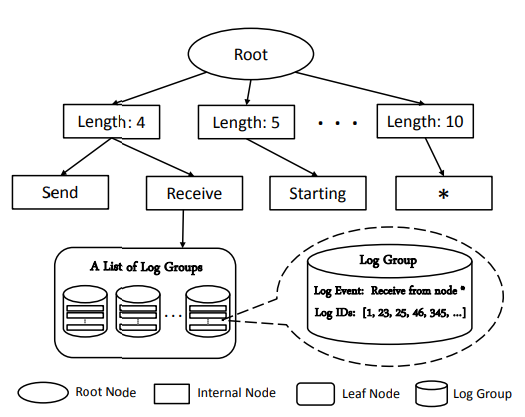
\includegraphics[scale=.5]{img/parse-tree-drain.PNG}}
            \caption{Structure of a simple parsing tree of depth $3$ in Drain \cite{drain2017}.}
            \label{parseTreeDrain}
        \end{figure}
        
    The algorithm consists of five steps: 
    
    \begin{enumerate}
        \item \textit{Preprocess by Domain Knowledge}. According to the empirical study on log parsing methods by He et al. \cite{logParsingEvaluation2016}, preprocessing improves parsing accuracy. Thus, when a new raw log message arrives, Drain will preprocess it with regular expressions provided by the user based on domain knowledge before constructing the actual parse tree. This may include frequently used variables, such as IP address, and any matched tokens will be removed. 
        
        \item \textit{Search by Log Message Length}. The next step is to build the parsing tree. The process is based on the assumption that log messages with the same log event can have the same log message length. Starting from the root node, each node in the first layer represents log groups whose log messages have different lengths. The message length is specified by the number of tokens. Cases where log messages with the same log event have different lengths can be handled by post-processing. For example, the path to the preprocessed log message \texttt{Packet has been sent} to a first layer node would be \textit{Length: 4}.
        
        \item \textit{Search by Preceding Tokens}. In the third step, the parsing tree is traversed to a leaf node in the second layer. In this step, it is assumed that the first tokens in a log message are likely to be constants. For example, in the log message \texttt{Packet has been sent}, the tree is traversed from the first layer node \textit{Length: 4} to the leaf node containing the internal node \textit{Packet}, since "Packet" is considered a constant. Therefore, the second layer contains nodes with unique first words. Depending on the \textit{depth} of the tree, there are more internal nodes which search by the tokens at the first, second, third... etc. position. However, sometimes a variable word may appear in the initial positions, such as \texttt{120 bytes received}. This is solved by considering only tokens that do not contain digits. If a token contains a digit, it matches a special internal node \textit{"*"}. 
        \item \textit{Search by Token Similarity}. After step 3, lists of log groups are contained in leaf nodes. Each log group has \textit{log event} and
        
        \textit{log IDs}. Log event is the template that describes the log messages of the group, and log IDs are the log IDs of the log messages in that group. Each log group contains log messages of the same length that start with the same word. In this step, Drain calculates the similarity between the log message and the log event of each log group. The similarity is calculated over each token position. The highest similarity score is compared to a predefined similarity threshold, which indicates whether the given log group is suitable.
        \item \textit{Update the Parse Tree}. In the last step, the log ID of the current log message is added to the most suitable log group from step $4$ and log event in the log group is updated (different tokens are replaced by wildcards *).
    \end{enumerate}

    \subsection{Summary} \label{parser_summary}
    In this section, we presented an overview of automated log parsing techniques and their representative tools. Table \ref{tab:logParsers} provides a summary of all log parsing tools we have reviewed in this paper. The tools are compared from different aspects that we considered important for our use case. \textbf{Mode} denotes the online or offline mode, while \textbf{Method} denotes the log parsing technique used by the tool. \textbf{Preprocessing} describes whether an additional manual preprocessing step is required. \textbf{Performance} categorizes tools into three levels based on their efficiency: high, medium, and low, as proposed in \cite{zhlhxzl2018}. Finally, it is of great importance for practical use that log parsing tools are freely available. Therefore, the last column is devoted to the \textbf{Open Source} characteristics of the existing tools.
    
    \begin{table}[t]
    \centering
    \resizebox{\textwidth}{!}{\begin{tabular}{|c|c|c|c|c|c|c|}
    \hline
    \textbf{Log Parsing Tool} & \textbf{Year} & \textbf{Mode} & \textbf{Method}         & \textbf{Preprocessing} & \textbf{Performance} &  \textbf{Open Source} \\ \hline
    SLCT             & 2003 & Offline & Frequent Pattern Mining & \xmark     & High     & \cmark         \\
    LogSig           & 2011 & Offline & Clustering              & \xmark      & Medium       & \xmark           \\
    IPLoM            & 2012 & Offline & Iterative Partitioning  & \xmark     & High        & \xmark           \\
    Drain            & 2017 & Online  & Fixed-depth tree        & \cmark    & High     & \cmark         \\ \hline
    \end{tabular}}
    \caption{Summary of automated log parsing tools}
    \label{tab:logParsers}
    \end{table} 
    
    After understanding and comparing the properties of different log parsing tools described in this section, as well as evaluating these tools in detail on different systems in the paper by Zhu et al. \cite{zhlhxzl2018}, we decided to use Drain. The benchmarking results showed that Drain is superior in terms of accuracy, robustness and efficiency. Moreover, its online nature is of great practical importance for our research, considering that the Motorola SmartConnect system is constantly subject to change. Also, we often work with smaller time intervals of data, so log lines generated in different time windows may result in a different event template set. Not having to provide the entire log dataset before parsing is an undeniable advantage.
